%%%%%%%%%%%%%%%%%%%%%%%%%%%%%%%%%%%%%%%%%%%%%%%%%%%%%%%%%%%%%%%
%%%  notes
%%%%%%%%%%%%%%%%%%%%%%%%%%%%%%%%%%%%%%%%%%%%%%%%%%%%%%%%%%%%%%%

\documentclass[onecolumn,fleqn,notitlepage,secnumarabic]{revtex4}

% special 
\usepackage{ifthen}
\usepackage{ifpdf}
\usepackage{float}
\usepackage{color}

% fonts
\usepackage{latexsym}
\usepackage{amsmath} 
\usepackage{amssymb} 
\usepackage{bm}
\usepackage{wasysym}


\ifpdf
\usepackage{graphicx}
\usepackage{epstopdf}
\else
\usepackage{graphicx}
\usepackage{epsfig}
\fi

% packages added by jarondl
%
%\usepackage{subfig}  %% causes odd captions
\usepackage{verbatim} % for multiline comments
\usepackage{natbib} % change the bibliography style 
\usepackage{fancybox} % allows putting boxes with borders
\usepackage{cmap}  % for making pdf mathmode searchable
%\usepackage{sectsty}
\usepackage[pdftitle={Notes by Jarondl}]{hyperref}  % for hyperlinks in biblio. should be called last?

\graphicspath{{figures/},{PROG/figures/}}


%%%%%%%%%%%%%%%%%%%%%%%%%%%%%%%%%%%%%%%%%%%%%%%%%%%%%%%%%%%%%%%%


% NEW 
\newcommand{\abs}[1]{\left|#1\right|}
\newcommand{\Prob}{\mbox{Prob}\,}
\newcommand{\erf}{\mbox{erf}\,}
\newcommand{\barline}[1]{#1}

% math symbols I
\newcommand{\sinc}{\mbox{sinc}}
\newcommand{\const}{\mbox{const}}
\newcommand{\trc}{\mbox{trace}}
\newcommand{\intt}{\int\!\!\!\!\int }
\newcommand{\ointt}{\int\!\!\!\!\int\!\!\!\!\!\circ\ }
\newcommand{\ar}{\mathsf r}
\newcommand{\im}{\mbox{Im}}
\newcommand{\re}{\mbox{Re}}

% math symbols II
\newcommand{\eexp}{\mbox{e}^}
\newcommand{\bra}{\left\langle}
\newcommand{\ket}{\right\rangle}

% Mass symbol
\newcommand{\mass}{\mathsf{m}} 
\newcommand{\Mass}{\mathsf{M}} 

% more math commands
\newcommand{\tbox}[1]{\mbox{\tiny #1}}
\newcommand{\bmsf}[1]{\bm{\mathsf{#1}}} 
%\newcommand{\amatrix}[1]{\matrix{#1}} 
\newcommand{\amatrix}[1]{\begin{matrix} #1 \end{matrix}} 
\newcommand{\pd}[2]{\frac{\partial #1}{\partial #2}}

% equations
\newcommand{\mylabel}[1]{\label{#1}} 
%\newcommand{\mylabel}[1]{\textcolor{blue}{[#1]}\label{#1}} 
\newcommand{\beq}{\begin{eqnarray}}
\newcommand{\eeq}{\end{eqnarray}} 
\newcommand{\be}[1]{\begin{eqnarray}\ifthenelse{#1=-1}{\nonumber}{\ifthenelse{#1=0}{}{\mylabel{e#1}}}}
\newcommand{\ee}{\end{eqnarray}} 

% arrangement
\newcommand{\drawline}{\begin{picture}(500,1)\line(1,0){500}\end{picture}}
\newcommand{\bitem}{$\bullet$ \ \ \ }
\newcommand{\Cn}[1]{\begin{center} #1 \end{center}}
\newcommand{\mpg}[2][1.0\hsize]{\begin{minipage}[b]{#1}{#2}\end{minipage}}
\newcommand{\mpgt}[2][1.0\hsize]{\begin{minipage}[t]{#1}{#2}\end{minipage}}
\newcommand{\putgraph}[2][width=0.30\hsize]{\includegraphics[#1]{#2}}

% more
%\newcommand{\Eq}[1]{Eq.\!\!~(\ref{#1})}
%\newcommand{\Fig}[1]{Fig.\!\!~\ref{#1}}  
\newcommand{\Eq}[1]{\textcolor{blue}{Eq.\!\!~(\ref{#1})}} 
\newcommand{\Fig}[1]{\textcolor{blue}{Fig.}\!\!~\ref{#1}} 
\newcommand{\hide}[1]{} %{\textcolor{red}{[hidden text]}} %{}
\newcommand{\rmrk}[1]{\textcolor{red}{#1}}


%%%%%%%%%%%%%%%%%%%%%%%%%%%%%%%%%%%%%%%%%%%%%%%%%%%%%%%%%%%%%%%%%%%%%%%%%%%

% extra math commands by jarondl
\newcommand{\inner}[2]{\left \langle #1 \middle| #2\right\rangle} % Inner product

%fminipage using fancybox package
\newenvironment{fminipage}%
  {\begin{Sbox}\begin{minipage}}%
  {\end{minipage}\end{Sbox}\fbox{\TheSbox}}


%%%%%%%%%%%%%%%%%%%%%%%%%%%%%%%%%%%%%%%%%%%%%%%%%%%%%%%%%%%%%%%%%%%%%%%%%%%

% Page setup
\setlength{\parindent}{0cm} 
\setlength{\parskip}{0.3cm} 

%%% Sections. The original revtex goes like this:
%\def\section{%
%  \@startsection
%    {section}%
%    {1}%
%    {\z@}%
%    {0.8cm \@plus1ex \@minus .2ex}%
%    {0.5cm}%
%    {\normalfont\small\bfseries}%
%}%
%\def\subsection{%
%  \@startsection
%    {subsection}%
%    {2}%
%    {\z@}%
%    {.8cm \@plus1ex \@minus .2ex}%
%    {.5cm}%
%    {\normalfont\small\bfseries}%
%}%
%%%%%%% And our version goes like this:
\makeatletter
\def\section{%
  \@startsection
    {section}%
    {1}%
    {\z@}%
    {0.8cm \@plus1ex \@minus .2ex}%
    {0.5cm}%
    {\Large\bf $=\!=\!=\!=\!=\!=\;$}%
}%
\def\subsection{%
  \@startsection
    {subsection}%
    {2}%
    {\z@}%
    {.8cm \@plus1ex \@minus .2ex}%
    {.5cm}%
    {\normalfont\small\bfseries$=\!=\!=\!=\;$}%
}%
%%%%%%%%%%  Here we deal with capitalization. The original revtex first, and then our version.
%\def\@hangfrom@section#1#2#3{\@hangfrom{#1#2}\MakeTextUppercase{#3}}%
%\def\@hangfroms@section#1#2{#1\MakeTextUppercase{#2}}%
\def\@hangfrom@section#1#2#3{\@hangfrom{#1#2}{#3}}%
\def\@hangfroms@section#1#2{#1{#2}}%
\makeatother




\renewcommand{\includegraphics}[2][]{\ \\ \ FIGURE: \ \\ \ }



%%%%%%%%%%%%%%%%%%%%%%%%%%%%%%%%%%%%%%%%%%%%%%%%%%%%%%%%%%%%%
%%%%%%%%%%%%%%%%%%%%%%%%%%%%%%%%%%%%%%%%%%%%%%%%%%%%%%%%%%%%%
\begin{document}

\title{Notes regarding LRT to VRH crossover}

\author{Yaron de Leeuw, Doron Cohen}
\date{\today}
\maketitle

%%%%%%%%%%%%%%%%%%%%%%%%%%%%%%%%%%%%%%%%%%%%%%%%%%%%%%%%%%%%%%%%%%%%%%%%%%%%%%%%%%%%%%%%%%%%
%%%%%%%%%%%%%%%%%%%%%%%%%%%%%%%%%%%%%%%%%%%%%%%%%%%%%%%%%%%%%%%%%%%%%%%%%%%%%%%%%%%%%%%%%%%

We consider 1D ($d{=}1$) or 2D ($d{=}2$) network systems whose dynamics is described 
by a rate equation, with transitions rates $w_{nm}$ that form a symmetric matrix.
For presentation purpose we regard the nodes of the network as {\em sites}, 
each having a location~$x_n$. In particular (but no exclusively) we are interested 
in a model where the rates depend exponentially on the distance 
between randomly distributed sites, namely $w_{nm}\propto \exp(|x_n-x_m|/\xi)$. 
It is natural to characterize such a system by a sparsity parameter~$s$ 
that reflects the connectivity of the network. In the above example 
the natural definition is $s=\xi/r_0$ where $r_0$ is the average distance 
between neighboring sites. 

The models that we address are related and motivated  
by various physical problems, for example: 
phonon propagation in disordered solids \cite{phn1,phn2,amir}; 
Mott hopping conductance \cite{mott,miller,AHL,pollak,VRHbook};
conductance of ballistic rings \cite{kbd};
energy absorption by trapped atoms \cite{kbw}. 
Optionally these models can be fabricated by combining oscillators: 
say mechanical springs or electrical RC elements.    
In all these examples the issue is to understand how 
the {\em transport} is affected by the {\em sparsity} of a network.  
If the rates are induced by a driving source, this issue can be phrased as  
going {\em beyond} the familiar framework of Linear Response Theory (LRT), 
as explained below.  

Our interest is focused in the diffusion coefficient $D$ that characterizes the 
long time dynamics of a spreading distribution. It can be defined or deduced 
either from the variance ${S(t) \sim Dt}$ or from the decay of the 
survival probability ${\mathcal{P}(t) \sim (D t)^{-d/2}}$. Hence it is 
related to the spectral properties of the transition rate matrix ${\bm{w}=\{w_{nm}\}}$.
Exploiting the formal analogy with a resistor network calculation \cite{miller},  
namely $w_{nm}$ are like connectors and $D$ is like conductivity, 
one realizes that $D$ is given by a semi-linear functional $D=D[\bm{w}]$ 
that has the property ${D[\lambda \bm{w}] = \lambda D[\bm{w}]}$, 
while in general ${D[\bm{w}^a+\bm{w}^b] > D[\bm{w}^a]+D[\bm{w}^b]}$ instead of equality.      

In 1D it is well known \cite{alexander} that $D$ can display an abrupt 
percolation-like transition from diffusive (${D>0}$) to sub-diffusive (${D=0}$) 
behavior as the sparsity parameter drops below the critical value ${s_c=1}$.   
The question arises whether such a transition happens also in 
higher dimensions. In \cite{amir} the spectral properties in the 2D case 
have been investigated very seriously, but the results were {\em inconclusive}  
as far as the question above is concerned.

It should be clear that there are two major routes in developing  
a theory for~$D$. Instead of deducing it from spectral properties 
as in \cite{amir}, one can try to find ways to evaluate it directly 
via a resistor network calculation \cite{miller}.
In \cite{kbd,kbw} this approach has been extended to handle matrices 
whose elements have log-wide rather than Gaussian 
distribution, leading to a generalized Variable Range Hopping (VRH) strategy. 
In what follows we pursue the same direction and obtain an 
improved Effective Range Hopping (ERH) estimate for~$D$.
Using this approach we show that in the 2D case, as $s$ becomes small, 
the functional $D[\bm{w}]$ exhibits a smooth crossover from LRT behavior  
to semi-linear VRH-like dependence.  


\begin{thebibliography}{99}


%%% Phn

\bibitem{phn1} 
S. R. Nagel, A. Rahman, G. S. Grest, 
Phys. Rev. Lett. 47, 1665 (1981).

\bibitem{phn2} 
W. Schirmacher, M. Wagener, 
Philos. Mag. B 65, 607 (1992).


\bibitem{amir} 
A. Amir, Y. Oreg, Y. Imry,
Phys. Rev. Lett. 105, 070601 (2010); 
%
Phys. Rev. B 77, 165207 (2008).


%%% VRH

\bibitem{mott} 
N.F. Mott, Phil. Mag. {\bf 22}, 7 (1970). 
\ N.F.~Mott and E.A.~Davis, 
Electronic processes in non-crystalline materials, 
(Clarendon Press, Oxford, 1971). 

\bibitem{miller}
A. Miller and E. Abrahams, Phys. Rev. {\bf 120}, 745 (1960).

\bibitem{AHL}
V. Ambegaokar, B. Halperin, J.S. Langer, 
Phys. Rev. B {\bf 4}, 2612 (1971). 

\bibitem{pollak}
M. Pollak, J. Non-Cryst. Solids {\bf 11}, 1 (1972).

\bibitem{VRHbook} 
B.I. Shklovskii and A.L. Efros, 
Electronic properties of doped semiconductors,
(Springer-Verlag Berlin Heidelberg 1984).


%%% Ours

\bibitem{kbd} 
%
S. Bandopadhyay, Y. Etzioni, D. Cohen,
Europhys. Lett. {\bf 76}, 739 (2006).
%
D. Cohen,
Phys. Rev. B {\bf 75}, 125316 (2007).
%
A. Stotland, T. Kottos, D. Cohen, 
Phys. Rev. B {\bf 81}, 115464 (2010). 


\bibitem{kbw}
%
A. Stotland, D. Cohen, N. Davidson, 
Europhys. Lett. {\bf 86}, 10004 (2009).
%
A. Stotland, L.M. Pecora, D. Cohen, 
Europhys. Lett. {\bf 92}, 20009 (2010);
Phys. Rev. E {\bf 83}, 066216 (2011).

%%% Results

\bibitem{alexander}
S. Alexander, J. Bernasconi, W. R. Schneider, R. Orbach, 
Rev. Mod. Phys. 53, 175 (1981).


\end{thebibliography}



%%%%%%%%%%%%%%%%%%%%%%%%%%%%%%%%%%%%%%%%%%%%%
\section{The model system}


We consider a system that is described by a rate equations 
%
\beq
\frac{dp_n(t)}{dt} = \sum_m w_{nm} p_m(t)
\eeq
%
We assume $w_{nm}=w_{mn}$, hence there is a formal analogy 
we a resistor network calculation. Our purpose is to calculate 
the diffusion coefficient~$D=D[\bm{w}]$, which is analogous to the 
calculation of {\em conductivity}.


Our interest are in networks that consists of sites 
that are distributed in space, locations $x_n$.
With each bond we associate an activation energy $\epsilon_{nm}>0$. 
By construction the rates rates are given by the following expression:
%
\beq
w_{nm} \ \ = \ \  w(|x_n-x_m|,\epsilon_{nm})  \ \ = \ \  w_0 \ \eexp{-\epsilon_{nm}} \ \eexp{-|x_n-x_m|/\xi} 
\ \ \ \ \ \ \ \mbox{[random site model]}
\eeq
%
In the 1D case we consider also the following banded lattice model
%
\beq
w_{nm} \ \ = \ \  w(|n-m|,\epsilon_{nm})  \ \ = \ \  w_0 \ \eexp{-\epsilon_{nm}} \ B(n-m)
\ \ \ \ \ \ \ \mbox{[banded lattice model]}
\eeq
% 
Below we define $r=|x_n-x_m|$ or $r=|n-m|$ depending on the context.
For flat band $B(r)=1$ for ${r \leq b}$, and zero otherwise,  
where $1{+}2b$ is the bandwidth. For a model with near-neighbor transitions only $b=1$.
The density of sites relative to some site is characterized  by a joint distribution function 
%
\beq\label{eq:density_distribution}
\rho(r,\epsilon)drd\epsilon \ \ = \ \ \frac{\Omega_d \, r^{d-1}dr}{r_0^{d}} \ f(\epsilon)d\epsilon,     
\ \ \ \ \ \ \ \ \Omega_d=2,2\pi,4\pi, \ \ \ \ \ \ \ \ f(\epsilon)=\mbox{uniform or normalized}
\eeq
%
The constant $r_0^d$ is the "unit volume", and it is defined by $Nr_0^d = L^d$, 
where $N$ is the number of sites, and $L^d$ is the volume of the system.
It is ${r_0=1}$ in the banded lattice model, 
while in the random site model it sets the units of length.
%  
For a uniform distribution of sites in energy space one may set ${f(\epsilon)=\const}$.
In particular in the finite temperature Mott problem ${f(\epsilon)= T/\Delta_0}$,  
where $\Delta_0$ is the local mean level spacing per unit volume.
In such case in each location there are infinitely many sites, 
but effectively only finite number of sites ($\sim T/\Delta_0$) 
is accessible per unit volume per attempted transition.  
Optionally one may assume an $f(\epsilon)$ that has a unit normalization, 
corresponding to a single site per unit volume. 
What we call below "infinite temperature case" refers to 
the special choice $f(\epsilon)=\delta(\epsilon)$. 
In the banded lattice model $f(\epsilon)$ reflects the size distribution 
of the in-band matrix elements of the perturbation matrix. 

In one dimension the random site model is qualitatively similar 
to a banded lattice model with near neighbor transitions (${b=1}$),
with the identification $\epsilon=r/\xi$,   
and $f(\epsilon) = s\exp(-s\epsilon)$, where $s \equiv \xi/r_0$. 
This implies that the the distribution of the rates is 
%
\beq
\tilde{f}(w) dw  \ \  =  \ \    \ [w < w_0] \, \frac{s \, w^{s-1} dw}{w_0^s}, 
\ \ \ \ \ \ \ \ s \equiv \xi/r_0
\eeq


%%%%%%%%%%%%%%%%%%%%%%%%%%%%%%%%%%%%%%%%%%%%%

\clearpage

%%%%%%%%%%%%%%%%%%%%%%%%%%%%%%%%%%%%%%%%%%%%%
\section{Exact results for the Chain model}

In the case of the chain model
using the notation $w_n=w_{n,n{-}1}$ 
and making the analogy with adding connectors in series 
the expression for $D$ is 
%
\beq
D \ \ = \ \ D[w_n] \ \ = \ \ \left( \frac{1}{N} \sum_n \frac{1}{w_n} \right)^{-1} 
\ \ = \ \ \frac{s-1}{s} \, w_0
\eeq
%
where the last equality is for the distribution of Eq(5).
In the sub diffusive regime (${0<s<1}$) the results 
for the survival probability and the spreading are 
%
\beq
S(t) \ \ &\propto& \ \ t^{2s/(1+s)}   \\ 
\mathcal{P}(t) \ \ &\propto& \ \ t^{-s/(1+s)}
\eeq

These results are summed up in the following figure:
\begin{figure}[H]
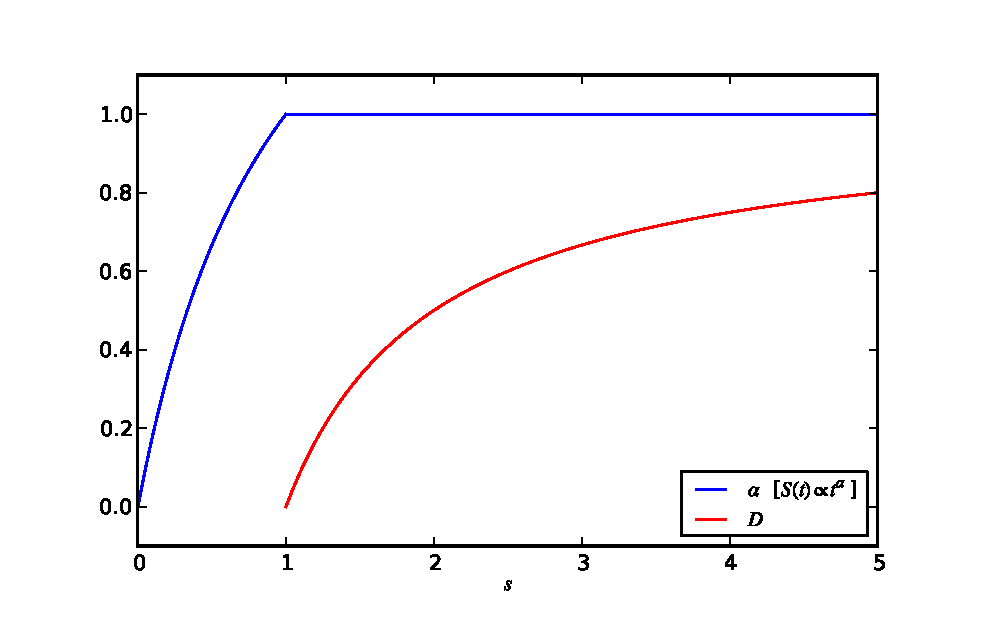
\includegraphics{alexander}
\end{figure}
%%%%%%%%%%%%%%%%%%%%%%%%%%%%%%%%%%%%%%%%%%%%%
\section{Linear response theory (LRT) estimate}

If we had an ordered lattice, then the exact result for $D$ would be 
%
\beq
D \ \ = \ \ D_{\tbox{LRT}}[\bm{w}]  \ \ = \ \ \frac{1}{4}\iint w(r,\epsilon) \ r^2  \ \rho(r,\epsilon) \ d\epsilon dr 
\eeq
%
This expression is strictly {\em linear}.
For the infinite temperature variation of 2D random site model we get  
%
\beq
D \ \ = \ \ 3\pi \, s^4 \, w_0
\eeq
%
This expression will not work for ${s<1}$ because sparse contribution 
of strongly coupled sites do not contribute to the transport. 
Only percolating trajectories do have a contribution. We are therefore urged 
to introduce approximation schemes that takes this connectivity 
issue into account.  
 

%%%%%%%%%%%%%%%%%%%%%%%%%%%%%%%%%%%%%%%%%%%%%
\section{Effective Range Hopping (ERH) estimate}

What we call Effective Range Hopping (ERH) estimate is based 
on the idea of finding a lower bound for $D$, taking the 
percolation threshold into account. We define the effective rate 
through the requirement 
%
\beq
\iint_{w(r,\epsilon)>w*} \rho(r,\epsilon)drd\epsilon \ \ = \ \ p_c, 
\ \ \ \ \ \ \ \ \ \mbox{with $p_c\sim 1/2$}
\eeq
%
Then we calculate $D$ as follows:
%
\beq
D \ \ = \ \ D_{\tbox{ERH}}[\bm{w}]  \ \ = \ \ \frac{1}{4}\iint \min\{w(r,\epsilon),w^*\} \ r^2  \ \rho(r,\epsilon) \ d\epsilon dr
\eeq
%
This is similar to the LRT estimate, with network that has $w_{nm}$ 
that are equal or smaller to the original values. The "suppressed" 
connector are those that are too sparse to form percolating trajectories. 
Note that this expression, as required, is {\em semi-linear} 
rather than linear [see explanation below].
For the infinite temperature variation of 2D random site model we get  
%
\beq
D \ \ \sim \ \ 3\pi \, s^4 \, \eexp{-\const/s} \, w_0, 
\ \ \ \ \ \ \ \ \ \ \ \const\sim 1 \mbox{(fitting)} 
\eeq


%%%%%%%%%%%%%%%%%%%%%%%%%%%%%%%%%%%%%%%%%%%%%
\section{Variable Range Hopping (VRH) estimate}

The ERH is similar to the generalized VRH procedure 
that we have introduced in previous publications.
We define below what we mean by generalized VRH. 
It would be clear that ERH gives in-fact a better (higher) 
lower bound compared with VRH. Namely, 
%
\beq
D_{\tbox{VRH}}[\bm{w}]  
\ \ < \ \ D_{\tbox{ERH}}[\bm{w}]
\ \ < \ \ D[\bm{w}]
\ \ < \ \ D_{\tbox{LRT}}[\bm{w}]
\eeq
%
The VRH is based on the idea to associate
with the range of the jump $r$ its typical 
energy cost $\epsilon(r)$. In the Mott problem 
the relation is $\epsilon(r) = (r_0/r)^d \Delta_0$, 
corresponding to the effective DOS in range~$r$. 
More generally the relation between $\epsilon$ and $r$ 
is determined through the equation 
%
\beq
\int_0^{\epsilon} \int_0^{r} \rho(r',\epsilon')  dr'd\epsilon' \  = \  p_c 
\ \ \ \ \ \ \ \ \leadsto \ \ \ \ \ \ \ \ 
\left(\frac{r}{r_0}\right)^d \ F(\epsilon) \ = \ p_c
\eeq
%
where $F(\epsilon)$ is the cumulative distribution function.
In words this equation asks what is the $\epsilon$~window that 
is required in order to guarantee that the particle will be able 
to find with probability of order unity an accessible site within 
a range~$r$. Larger jumps allow smaller cost. 
Then we calculate $D$ as follows: 
%
\beq
D \ \ = \ \ D_{\tbox{VRH}}[\bm{w}]  \ \ = \ \ 
\frac{1}{4}\iint \Theta\left\{ (r/r_0)^d F(\epsilon) - p_c \right\} \ w(r,\epsilon) \ r^2  \ \rho(r,\epsilon) \ d\epsilon dr
\eeq
%
This integral excludes all those transitions that are not likely to connect. 
It is in the same spirit as the ERH estimate, but gives a lower result 
for two reasons: (i) compared with the ERH integral a larger portion of 
the $drd\epsilon$ plane is modified. (ii) The modification in this portion 
is exclusion instead of flattening to a lower value.
However, it should be realized that in the Mott problem the VRH 
integral is dominated by the vicinity of the optimal point ${(r^*,\epsilon^*)}$, 
where $\epsilon^*=\epsilon(r^*)$ is the same as in the ERH. 
Therefore, in the Mott problem, both estimates give essentially the same result.


%%%%%%%%%%%%%%%%%%%%%%%%%%%%%%%%%%%%%%%%%%%%%
\section{The semi-linear response perspective}

Assume that the rates $w_{nm}$ are induced 
by a driving source that has spectral content $\tilde{S}(\omega)$. 
Say that the rates are determined by the Fermi golden rule:
%
\beq
w_{nm} \ \ = \ \ \tilde{S}(E_n-E_m) |V_{nm}|^2
\eeq
%
Accordingly we can write instead of~$D=D[\bm{w}]$ a relation~$D=D[\tilde{S}(\omega)]$.
This relation is in general semilinear. This means that only the first property below 
is satisfied, not the second one.
%
\beq
D\big[ \lambda \tilde{S}(\omega)\big]  \ \ &=& \ \  \lambda \ D\big[\tilde{S}(\omega)\big] 
\\
D\big[\tilde{S}_a(\omega) + \tilde{S}_b(\omega)\big]  \ \ &=& \ \  D\big[\tilde{S}_a(\omega)\big] + D\big[\tilde{S}_b(\omega)\big]
\eeq
%
A typical situation is that the driving is "on top" of a bath. Namely 
%
\beq
\tilde{S}(\omega) \ \ = \ \ \tilde{S}_{\tbox{bath}}(\omega) + \tilde{S}_{\tbox{driving}}(\omega)
\eeq  
%
In such case we can linearize~$D=D[\tilde{S}(\omega)]$, and then we get 
linear-response. Otherwise the response is typically semi-linear rather than linear. 



%%%%%%%%%%%%%%%%%%%%%%%%%%%%%%%%%%%%%%%%%%%%%
\section{Numerical extraction of $D$}


We use the well known fact that the survival probability 
is related to the eigenvalues of $w_{nm}$ through the relation
%
\beq
\mathcal{P}(t) \ \ = \ \ \frac{1}{N}\sum_\lambda \eexp{\lambda t} \ \ \equiv \ \ \int_0^{\infty} g(\lambda)d\lambda \ \eexp{\lambda t}
\eeq
%
If the system is diffusive (see \eqref{eq:surv_d})
%
\beq
  \mathcal{P}(t) \quad \sim \quad  \frac{1}{\left({4\pi D t}\right)^{d/2}} 
  \qquad\qquad[r_0^d=1]
\eeq
%
If follows that $D$ can be deduced from 
the asymptotic behavior in the ${\lambda\rightarrow 0}$ limit  
%
\beq
\int_0^\lambda g(\lambda')d\lambda' \quad = \quad \frac{\Omega_d}{d}\left[\frac{\lambda}{4\pi^2 D}\right]^{d/2}
\eeq
%
for large $\lambda$ we expect $g(\lambda)$ to coincide 
with the distribution of the decay rates $\gamma_n=\sum_{m}w_{mn}$, 
reflecting localized modes.



%%%%%%%%%%%%%%%%%%%%%%%%%%%%%%%%%%%%%%%%%%%%%
\section{Additional sections}

Mechanical and electrical analogs.

Regarding $D$ as conductivity.

Relation between $S(t)$ and $P(t)$ - simplify as in QM lecture notes.

Expressions for $P(t)$ in case of diffusion 1D and 2D

Remark about aging.

Spectral properties of [aaa...] and for [abab...] lattice

Spectral properties in 1D

Spacing distribution $P(r)$ in $d$ dimensions.

Implied $P(w)$ in $d$ dimensions. 

Analysis of the "random site" model (LRT to ERH crossover) 

Analysis of banded matrices (LRT to ERH crossover)

The errata KBD model. 


%%%%%%%%%%%%%%%%%%%%%%%%%%%%%%%%%%%%%%%%%%%%%%%%%%%%%%%%%%%%%%%%%%%%%%%%%%%%%%%%%%%%%%%%%%%%
%%%%%%%%%%%%%%%%%%%%%%%%%%%%%%%%%%%%%%%%%%%%%%%%%%%%%%%%%%%%%%%%%%%%%%%%%%%%%%%%%%%%%%%%%%%

\clearpage

\section{ERH calculation}
Let us do the ERH calculation for our specific case where $w =w_0 e^{-\frac{r}{s}}$, and $\rho(r) = 2\pi r$ \eqref{eq:density_distribution}.
%
\begin{align}
  \iint_{w(r,\epsilon)>w*} \rho(r,\epsilon)drd\epsilon \quad &= \quad p_c, \\
  \int_0^{r^*} 2\pi r dr \quad &=\quad p_c \\
  r^*  &= \sqrt\frac{p_c}{\pi}
\end{align}
%
Then we calculate $D$ as follows:
%
\begin{align}
  D_{\tbox{ERH}}[\bm{w}] \quad&=\quad \frac{1}{4}\iint \min\{w(r,\epsilon),w^*\} \ r^2  \ \rho(r,\epsilon) \ d\epsilon dr \\
  &= \frac{1}{4}\int_0^{r^*} w^* r^2\rho(r) dr  + \frac{1}{4}\int_{r^*}^\infty w(r) r^2\rho(r)dr \\
  &= \frac{1}{4}\int_0^{r^*} w^* r^2 2\pi rdr  + \frac{1}{4}\int_{r^*}^\infty w_0e^{-\frac{r}{s}} r^2 2\pi rdr \\
  &=  \frac{\pi}{8}w_0 e^{-\frac{r^*}{s}}{r^*}^4 + \frac{\pi}{2} w_0  e^{-\frac{r^*}{s}}\left( \left(\frac{r^*}{s}\right)^3 + 3\left(\frac{r^*}{s}\right)^2 + 6\left(\frac{r^*}{s}\right) +6 \right) s^4 \\
  &=  e^{-\frac{r^*}{s}}\frac{\pi}{2} w_0\left[\frac{1}{4}{r^*}^4 +  {r^*}^3 s + 3{r^*}^2 s^2 + 6r^*s^3 +6 s^4  \right]
\end{align}
%%%%% \int_y^\infty x^3 exp(-x) = exp(-y)(y^3 + 3y^2+ 6 y + 6)
%
When $r^* \rightarrow 0$, the solution converges to the known LRT solution: 
\beq
  D_{\tbox{ERH}}[\bm{w}] = 3\pi w_0 s^4 
\eeq

%%%%%%%%%%%%%%%%5
\section{Expressions of $P(t)$ and $S(t)$ in the case of diffusion in $1d$ and $2d$}
We define 
\beq
  S(t) = <r^2(t)> = 2Dt
\eeq
For an isotropic $d$-dimensional system, there is no correlation between the different axes. We can therefore seperate $S(t)$ to 
%
\beq 
  S(t) =<r^2(t)> = < \left(\sum_{i=1}^d x_i(t) \right)^2 > = \sum_{i=1}^d <x_i(t)^2> = d<x^2(t)>
\eeq
The normalized $d$ dimensional gaussian is:
%
\beq
  \prod_{i=1}^d \frac{1}{\sqrt{2\pi <x_i^2> }}e^{-\frac{x_i^2}{2<x_i^2>}}
\eeq
%
Whereby we obtain:
%
\beq\label{eq:surv_d}
  \mathcal{P}(t) = (4\pi D t)^{-d/2}
\eeq
%

\section{Introduction}
This work concerns the survival probality and spreading (defined in section \ref{sec:definitions}) for systems with multiple intercontected sites. We will study which physical and mathematical properties are necessary to describe the system. The systems are defined using the transition rates between sites (and sometimes the energy of the sites). Some sort of random distribution is used for building th systems, either by randomly setting the transition rates themselves, or by randomly positioning them in space, obtaining the transition rates from their distances. These physical systems are mapped to matrices, which are then further studied. The matrices have random origin, but are not completely random, due to physical or topological considirations.


In regular diffusion there is a known relation between the survival probability and the diffusion. 
A known solution for the diffusion constant in a nearest neighbor network is \cite{Derrida:1983}:
\begin{align}
D=\overline{w}_{harmonic} =(\overline{w^{-1}})^{-1}=\left(\frac{1}{N}\sum\frac{1}{w_n}\right)^{-1}
\end{align}

%%%%%%%%%%%%
\section{Questions}
\begin{itemize}
    \item Is the known relation $\mathcal{P}(t) \sim \frac{1}{\sqrt{S(t)}}$ general, and does it hold for more than two dimensions?
    \item Do geometrical and topological considirations matter, or is the rate distribution enough to find the survival and spreading?
    \item Could a resistor network calculation be the generalization of Alexander's solution (see section {sec:alexander}) for more than $1d$ (Quasi $1d$ or even $d>1$?
    \item What are the implications of different site energies, and does the VRH method address them correctly?
\end{itemize}
%%%%%%%%%%%%
\section{Tentative working plan}
Several systems of interest are defined in section \ref{sec:sys_of_interest}. With those systems 
\begin{itemize}
    \item Solve $1d$ nearest neighbors problems, analytically, numerically, and using the resistor network method. The numerical solution is based on finding the eigenvalues.
    \item Solve quasi-1d and strip systems.
    \item Analyze $2d$ systems, analytically and numerically.
    \item VRH: Variable-Range-Hopping, insert different energies for the sites, 
    \item Resistor network calculation \ref{sec:res_net}. Could a resistor network calculation be the generalization of Alexander's solution for more than $1d$ (Quasi $1d$ or even $d>1$?

\end{itemize}

%%%%%%%%%%%%%%%%%%%%%%%%
\section{definitions}\label{sec:definitions}
\begin{description}
    \item[Site probability - $P_n(t)$ : ] The probability to be in site $n$ at time $t$.
    \item[Survival probability - $\mathcal{P}(t)$ : ] The probability to remain in the starting site. If the initial condition was $P_0(0)=1$, $P_i(0)=0 \textrm{  for  } i\neq 0$, then $\mathcal{P}(t)= P_0(t)$
    \item[Spreading - $S(t)$ : ] The squared width (second moment) of the probability distribution. $S(t) \equiv \sum_n n^2 P_n -\left(\sum_n n P_n\right)^2$. 
    \item[Diffusion coefficient - $D$ : ] The long term ratio of spreading to time, with $S(t) \sim 2Dt$.
    \item[Rate matrix - $W_{ij}$ : ] A matrix describing the transition rates between sites. $W_{ij}$ is the rate of transitions from site $j$ to site $i$.
    \item[Probability conserving matrix : ]\label{def:prob_conserv} A matrix where the sum of each and every row is zero - $\sum_i W_{ij} = 0 \qquad \forall j$. This relates to conserving probability if this matrix is a rate matrix.
    \item[Banded matrix, with width $b$ : ] A matrix that has non zero values only within the first $b$ off diagonals, meaning $2b+1$ diagonals with values.
\end{description}


%%%%%%%%%%%%%%%%%%%%%%%%%%%%%%%
\section{Rate equation}

The basic model is of a particle distributed among many sites. The particle moves from site to site, with a transition rate matrix $W_{ij}$. Then, the probability to find the particle at a given site $i$, denoted $P_i$, obeys the rate equation:
\begin{align}
\frac{dP_n(t)}{dt} = \sum_m W_{nm}P_m(t)
\end{align}
We can generally describe a system by defining its transition matrix $W_{ij}$.

%%%%%%%%%%%%%%%%%%%%%%%%
\section{Systems of interest}\label{sec:sys_of_interest}

In the following sections we will describe several systems by defining their transition matrices. Unless stated otherwise, all the matrices are symmetric and probability conserving as defined previously \ref{sec:definitions}. The rates are obviously non negative.

%%%%%%%%%%%%%%%%%%%%%%%%%
\subsection{One dimensional nearest neighbor systems with wide distributions}

This class of systems has only nearest neighbor transitions, with non zero rates only on the first off diagonals. The rate distribution is wide, say $P(w) \sim \textrm{log wide}$.


If the transition rates are $w_1,w_2,w_3,...$, the matrix looks like this:
\begin{align}
W = 
\begin{pmatrix}
-w_1  & w_1 \\
w_1  & -w_1-w_2 &  w_2 \\
 & w_2 & -w_2-w_3 &  w_3 \\
& & w_3 & -w_3-w_4 & \; w_4 \\
& & & \ddots &\ddots&\;\;\ddots
\end{pmatrix}
\end{align}
%%%%%%%%%%%%%%%%%%%%%%%%%
\subsection{One dimension, beyond nearest neighbors}

This system has non zero rates to sites beyond the nearest neighbors. The largest distance with non zero rates will define the matrix bandwidth $b$.

%%%%%%%%%%%%%%%%%%%%%%%%%
\subsection{Quasi one dimensional - strip}

This system is two dimensional, but one of the dimensions is very small compared to the other. This matrix will also be banded.

%%%%%%%%%%%%%%%%%%%%%%%%%
\subsection{Two or higher dimensions}

This class of systems has the sites in a two (or more) dimensional system. An added difficulty is that there is more then one coordinate, so that there are several ways to map this to 1d vectors.

%%%%%%%%%%%%%%%%%%%%%%%%%
\subsection{Variable site energy}

Contrary to all the previous systems, here the energy per site is not constant. We can \cite{Ambegaokar:1971} accommodate for this, by including Boltzmann's factor in the transition rates. Another consequence is that the transition rates is not symmetric.

%%%%%%%%%%%%%%%%%%%%%%%%%%%%%%%
\section{The relation between the survival probability and the eigenmode distribution}
The matrix has eigenmodes $V_\lambda$ with eigenvalues $\lambda$. 
We define a standard inner product :
\begin{align}
\inner{A}{B} = \sum_{ii} A_iB_i
\end{align}
Then we can write the probability vector $P$ as a sum of the normalized eigenmodes.
\begin{align}
P_n(t) = \sum_\lambda \inner{P(t)}{V_\lambda}{V_\lambda }_n = \sum_\lambda C_\lambda(t) {V_\lambda}_n
\end{align}
Where we have defined $C_\lambda(t)\equiv \inner{P(t)}{V_\lambda}$.

The rate equation becomes
\begin{align}
&\sum_\lambda \left( \frac{dC_\lambda(t)}{dt}{V_\lambda}_n - C_\lambda(t)\sum_m W_{nm}{V_\lambda}_n \right)= \sum_\lambda \left( \frac{dC_\lambda(t)}{dt} - \lambda C_\lambda(t)\right){V_\lambda}_n =0\\
&C_\lambda(t) = C_\lambda(0)e^{\lambda t}\\
&P_n(t) = \sum_\lambda C_\lambda(t) {V_\lambda}_n = \sum_\lambda  C_\lambda(0)e^{\lambda t} {V_\lambda}_n 
\end{align}
The survival probability is defined as the probability to remain in a specific site. If we begin with a probability vector whose only non zero element is $P_i(0)=1$, the corresponding $C_\lambda(0)$s will be:
\begin{align}
C_\lambda(0) = \inner{P(0)}{V_\lambda}= {V_\lambda}_ito
\end{align}
And then the survival probability will be:
\begin{align}
\mathcal{P}_i(t) = P_i(t) = \sum_\lambda  C_\lambda(0)e^{\lambda t} {V_\lambda}_i=\sum_\lambda ({V_\lambda}_i)^2 e^{\lambda t} 
\end{align}
The mean survival probability will be:
\begin{align} \label{eq:surv_eigenvalues}
\mathcal{P}(t) = \sum_i \frac{1}{N} P_i(t)=\sum_i \frac{1}{N} \sum_\lambda ({V_\lambda}_i)^2 e^{\lambda t}  =\frac{1}{N}\sum_\lambda e^{\lambda t} = \int g(\lambda) e^{\lambda t}
\end{align}
Where $g(\lambda)$ stands for the density of eigenvalues. This last results means that the survival probability is the Laplace transform of the eigenvalue distribution.


%%%%%%%%%%%%%%
\section{The relation between the diffusion coefficient and the survival probability}
If $D$ exists, the long time decay of $\mathcal{P}(t)$, according to Alexander et al \cite{Alexander:1981:RMP}, (and consistent with the scaling hypothesis $\mathcal{P}(t)\sqrt{S(t)} \propto 1$) is:
\begin{align}
    \mathcal{P}(t) = \frac{1}{\sqrt{4\pi D t}} \\
    g(\lambda) = \mathcal{L}^{-1}[\mathcal{P}(t)] = \mathcal{L}^{-1}\left[\frac{1}{\sqrt{4\pi D t}}\right]
\end{align}
Where $\mathcal{L}^{-1}$ is the inverse Laplace transform, (The Bromwich integral).
\begin{align}
    g(\lambda) = \mathcal{L}^{-1}\left[\frac{1}{\sqrt{4\pi Dt}}\right] = \frac{1}{\sqrt{4\pi^2 D\lambda}} \\
    \int_0^\lambda g(\lambda')d\lambda' = \sqrt{\frac{\lambda}{\pi^2 D}}
\end{align}

%%%%%%%%%%%%%%%%%55
\section{The harmonic mean of log normal distribution}
The harmonic mean of the log normal distribution with normal width $\sigma$ is given by:
\begin{align}
\left(\frac{1}{N}\sum\frac{1}{w_n}\right)&= \int_{-\infty}^\infty \frac{1}{\sqrt{2\pi\sigma^2}}e^{-\frac{x^2}{2\sigma^2}} \frac{1}{e^x} dx  = \int_{-\infty}^\infty \frac{1}{\sqrt{2\pi\sigma^2}}e^{-\frac{x^2}{2\sigma^2}-x} dx \\
&= \int_{-\infty}^\infty \frac{1}{\sqrt{2\pi\sigma^2}}e^{-\frac{\left(x-\sigma^2\right)^2}{2\sigma^2}+\frac{\sigma^2}{2}} dx = e^{\frac{\sigma^2}{2}}\\
\left(\frac{1}{N}\sum\frac{1}{w_n}\right)^{-1} = e^{-\frac{\sigma^2}{2}}
\end{align}
The generalization for $\mu\neq 0$ is :
\begin{align}
\overline{w}_{harmonic} = e^{-\frac{\sigma^2}{2}+\mu}
\end{align}

%%%%%%%%%%%%%%%%%%%%%%%%%
\section{Solving nearest neighbor alternating transition rates analytically}
In this section I solve the alternating transition rates problem exactly.

We can think of a model where every second transition is different, so the transitions are a,b,a,b,a,b... And the matrix is:
\begin{align}
W = 
\begin{pmatrix}
-a  & a \\
a  & -a-b &  b \\
 & b & -a-b &  a \\
& & a & -a-b & \; b \\
& & & \ddots &\ddots&\;\;\ddots
\end{pmatrix}
\end{align}
The diffusion coefficient according to \ref{eq:diff} should be:
\begin{align}\label{eq:D_alter}
D = \left(\frac{1}{N}\sum\frac{1}{w_n}\right)^{-1} = \frac{2}{\frac{1}{a} + \frac{1}{b}} = \frac{2ab}{a+b}
\end{align}

Applying the eigenvalue equation to this matrix gives us two inidical equations, for even and odd $n$'s. If we take an odd $n$ the equations are:
\begin{align}
a {V_\lambda}_n - (a+b+\lambda){V_\lambda}_{n+1} + b {V_\lambda}_{n+2} =0  \\
b {V_\lambda}_{n+1} - (a+b+\lambda){V_\lambda}_{n+2} + a {V_\lambda}_{n+3} =0 
\end{align}
The solution with real eigenmodes is rather cumbersome, but the eigenvalues found by any set of orthogonal eigenmodes have to be the same. So for purely analytical reasons we find the eigenvalues with complex eigenmodes, although they have no meaning in our model.


The eigenvalues for this matrix can be found analytically, using Bloch's theorem. The solution for a periodic structure with a unit cell is ${V_\lambda}_n = e^{ikn} u(x)$ where $u(x)$ is a function with the periodicity of the unit cell. In our case this simplifies to:
\begin{align}
{V_\lambda}_n = \begin{cases}e^{ikn} c_1 \; &, \text{n odd} \\ e^{ikn} c_2 \; &, \text{n even} \end{cases}
\end{align}
Periodic boundary conditions dictate $k=\frac{2\pi}{N}m$ where $m$ is an integer.

When we apply the eigenvalue equation to this vector ($WV_\lambda = \lambda V_\lambda$), we obtain two linear equations:
\begin{align}
ac_1e^{-ik}   -(a+b)c_2 +bc_1e^{ik} &= \lambda c_2 \\
bc_2e^{-ik}   -(a+b)c_1 +ac_2e^{ik} &= \lambda c_1 
\end{align}
The solution for $\lambda$ is
\begin{align}
(a+b+\lambda)^2 = a^2+b^2+2ab\cos 2k \\
\lambda = -(a + b) \pm \sqrt{a^2+b^2+2ab\cos 2k}  \label{eq:abab_eigenvals}
\end{align}
We are interested in the eigenvalues close to zero, which means taking the plus sign, and $k\ll 1$:
\begin{align}
\lambda \approx -(a + b) + \sqrt{a^2+b^2+2ab(1-2k^2)} = -(a+b) +(a+b)\sqrt{1 - \frac{4abk^2}{(a+b)^2}}\approx \frac{2abk^2}{a+b}
\end{align}
The $k$'s are $k=\frac{2\pi}{N}m$, but with degeneracy of $2$ ($\pm k$ give the same result) and therefore the cumulative eigenvalues are:
\begin{align}
\sqrt{\lambda\frac{a+b}{2ab}}\frac{N}{\pi}
\end{align}
Or, using the diffusion coefficient we have found in \eqref{eq:D_alter}:
\begin{align}
\sqrt{\frac{\lambda}{D}}\frac{N}{\pi}
\end{align}

Now that we have the eigenvalues, we may use equation \ref{eq:surv_eigenvalues} to find the survival probability as a function of time:
\begin{align}
\mathcal{P}(t) =\int g(\lambda) e^{\lambda t} = \frac{1}{\sqrt{4 \pi D t}}
\end{align}



%%%%%%%%%%%%%%%%%%%%%%%%%%%%%%%%%%%%%
\section{The relation between the eigenvalue distribution and the transition matrix}
In the supplementary material of \cite{Amir:2010:PRL} the moments of the distribution of the eigenvalues are found. 

If we define $D$ as the diagonalized matrix $W$ as in $W=UDU^{-1}$, we have
\begin{align}\label{eq:eig_moments}
\sum_\lambda \lambda^k = Tr (D^k) = Tr(UDU^{-1}UDU^{-1}UDU^{-1}UDU^{-1}...) = Tr (W^k)
\end{align}
So the exponent $k$ of the matrix $W$ is equal to the $k^{th}$ moment of the distribution of the eigenvalues. If one can find the exponents of the matrix, he can find the moments of the distribution, and hopefully the distribution itself. 


%%%%%%%%%%%%%%
\section{Solving the spacing distribution for uniformly random points in d dimensions} \label{subsec:euclid}
Random Euclidean distance matrices were widely researched \cite{Mezard:1999:NPB}, [insert more refs..]. Amir et al \cite{Amir:2010:PRL} have studied a model with the exponents of euclidean distances. They obtain the survival probability by finding the distribution of the eigenvalues, using the idea of \ref{eq:eig_moments}. 

In one dimension, the transition rates are related to the distance between points distributed uniformly, with density $n$. The nearest neighbor distribution can be considered as the probability for no neighbor at $x'<x$, and a neighbor at $x<x'<x+dx$. Because the points are distributed uniformly, the probability for no neighbors at a small interval $\Delta x$ is :
\begin{align}P_0(\Delta x) = (1-n\Delta x) \end{align}
So for a larger interval, we can divide $x$ to $N$ parts:
\begin{align}P_0(x) = \lim_{N\rightarrow \infty}(1-\frac{nx}{N})^N = e^{-n x} \end{align}
The probability for a neighbor at $x<x'<x+dx$ is:
\begin{align}P_1(x<x'<x+dx) = n dx \end{align}
So the probability for a nearest neighbor between $x$ and $x+dx$ is:
\begin{align}P_{NN}(x< x'<x+dx) = P_0(x'<x)\cdot P_1(x<x'<x+dx) = e^{-n x}ndx \end{align}
And the distribution density functions is:
\begin{align} f(x) = e^{-n x}n\end{align}

For higher dimensions, if we assume that site density is constant (denoted $n$), then the probability for no neighbors in volume $V(r)$ is:
\begin{align} P_0( V(r)) = e^{-nV(r)}\end{align}
So the cumulative probability for the nearest neighbor distance to be less than $r$ is:
\begin{align} F (r) = 1-P_0(V(r)) = 1- e^{-nV(r)} \end{align}
The probability density is the derivative of the cumulative probability:
\begin{align} f(r) = \frac{dF(r)}{dr} =   e^{-nV(r)} n \frac{dV(r)}{dr} \end{align}
For two dimensions:
\begin{align} f(r) = e^{-n \pi r^2}n2\pi r \end{align}
For three dimensions:
\begin{align} f(r) = e^{-n \frac{4\pi}{3} r^3}n4\pi r^2 \end{align}
Amir et al. \cite{Amir:2010:PRL} come to the same equation in their supplementary material:

%%
\begin{fminipage}{\textwidth}
\begin{align}P_{nn}(r)=\frac{d
V_d}{r_{nn}} {(r/r_{nn})}^{d-1} e^{-V_d {(r/r_{nn})}^d}\end{align} 
where $V_d$ is the volume of a $d$ dimensional sphere and $r_{nn}$ is the
average nearest-neighbor distance.
\end{fminipage}

In our notation (replacing $V_d$ with the more conventional $\frac{\Omega_d}{d}$ ), we can write it as:
\begin{align} f(r) = e^{-n \frac{\Omega_d}{d} r^d} n\Omega_d r^{d-1} \end{align}

%%%%%%%%%%%%%%%%%%%%%%%%%%%%%%%%%%%%%%
\section{Finding the transition rate distribution for $w= e^{-r/ \xi}$, with random points}
We can change the random variable from $r$ to $w= e^{-r/ \xi}$, with $0<w<1$:
\begin{align}
    &|f_w(w)dw| = |f_r(r)dr| \\
    &f_w(w) = f_r(r)\left|\frac{dr}{dw}\right| = f_r(-\xi \ln w)\frac{\xi}{w} = e^{-n \frac{\Omega_d}{d} (-\xi\ln w)^d} n\Omega_d (-\xi\ln w)^{d-1}\frac{\xi}{w} \\
    &f_w(w) \sim \frac{|\ln w|^{d-1}}{w} e^{-|\ln w|^d}
\end{align}
In $1d$ that becomes:
\begin{align} f(w)= e^{n \xi\ln w} \frac{n\xi}{w} = w^{n\xi-1}n\xi\end{align}
Which matches Alexander's $\alpha = 1-n\xi$, and therefore should have survival of $\mathcal{P}(t)\propto t^{-\frac{1-\alpha}{2-\alpha}}= t^{-\frac{n\xi}{1+n\xi}}$. This result appears also in Amir's article.



For $2d$:
\begin{align} f(w) = e^{-n \pi (-\xi\ln w)^2} n 2\pi  (-\xi\ln w)\frac{\xi}{w}\end{align}

The diffusion coefficient is given by $\left(\overline{(w^{-1})}\right)^{-1}$:
\begin{align}
    & \overline{(w^{-1})} = \int_0^\infty \frac{1}{w} e^{-n \frac{\Omega_d}{d} r^d} n\Omega_d r^{d-1} dr = \int_0^\infty e^{-n \frac{\Omega_d}{d} r^d} n\Omega_d r^{d-1}e^{r/\xi} dr 
\end{align}
For $d>1$ this integral converges. If the naive $1d$ calculation holds, normal diffusion should occur.

Amir also finds the eigenvalue distribution (using the idea of equation \eqref{eq:eig_moments} ):

%%
\begin{fminipage}{\textwidth}
\begin{align} P(\lambda)=  \frac{\epsilon^d d V_d /2
(-\rm{log}(-\lambda/2))^{d-1} e^{-\frac{V_d}{2} \epsilon^d
(-\rm{log}(-\lambda/2))^d}}{\lambda} \end{align}


The cumulative $C(\lambda)$ of this distribution takes a
particularly simple form: 
\begin{align} C(\lambda)\equiv \int_\lambda^0
P(\lambda)d\lambda= e^{-\frac{V_d}{2} \epsilon^d
(-\rm{log}(-\lambda/2))^d} \end{align}
\end{fminipage}
Or in our notation:
\begin{align} C(\lambda)= e^{-\frac{\Omega_d}{d} n\xi^d \left( -\log(\frac{\lambda}{2})\right)^d}  \end{align}
In 2D that becomes:
\begin{align} C(\lambda) = e^{-\pi n\xi^2 \left(\log(\frac{\lambda}{2})\right)^2 } \end{align}
This cumulative distribution is the same as the log-normal probability distribution. 

%%%%%%%%%%%%%%%%%%%%%%
\section{The survival and spreading for the one dimensional problem}\label{sec:alexander}
We present the survival and spreading for several cases of 1d systems, based on the work by \textcite{Alexander:1981:RMP}.

Three classes are classified:
\begin{align} 
    &\mathrm{(a) : }\qquad (\overline{w^{-1}})^{-1} < \infty  \\
    &\mathrm{(b) : }\qquad P(w)\rightarrow \mathrm{const} \qquad\mathrm{as}\qquad w \rightarrow 0 \\
    &\mathrm{(c) : }\qquad P(w) = 
        \begin{cases} 
            (1-\alpha)w^{-\alpha} , & 0\le w \le 1 \\
            0, & \mathrm{otherwise}
        \end{cases}
        \qquad\mathrm{with}\qquad 0<\alpha<1
\end{align}
For two of the three classes the survival at $w\rightarrow 0$ and $t\rightarrow \infty$ are (6.13) [Where $D=(\overline{w^{-1}})^{-1}$ ]:
\begin{align}
&\mathrm{(a) : }\qquad \mathcal{P}(t) \approx \sqrt{\frac{1}{4\pi D t}}  \\
&\mathrm{(c) : }\qquad \mathcal{P}(t) \propto t^{-\frac{1-\alpha}{2-\alpha}}
\end{align}
The spreading is defined by (7.3):
\begin{align}\label{eq:spreading}
     S(t) = \overline{x^2(t)} = \sum_n n^2 P_n(t) 
\end{align}
And it is solved (7.18):
\begin{align}
    &\mathrm{(a) : }\qquad S(t) \approx 2Dt  \\
    &\mathrm{(b) : }\qquad S(t) \propto \frac{t}{\ln t}  \\
    &\mathrm{(c) : }\qquad S(t) \propto t^{2\frac{1-\alpha}{2-\alpha}}
\end{align}
Using a scaling hypothesis , he claims:
\begin{align}\label{eq:scaling_hypo}
S(t) \propto \left(\mathcal{P}(t)\right)^{-2} \qquad \mathrm{as}\qquad t\rightarrow \infty
\end{align}

%%%%%%%%%%
\section{Higher dimension considerations}
To solve the problem in higher dimensions, we label the sites with a 1d coordinate, and solve the matrix.

The claim in \eqref{eq:eig_moments} that $\sum_\lambda \lambda^k = Tr (W^k)$, is still be valid in higher dimensions. Therefore, the survival probability should stay the same.

The interesting question regards the spreading. If the hypothesis $S(t) \propto \left(\mathcal{P}(t)\right)^{-2}$ \eqref{eq:scaling_hypo} holds, the spreading should also stay the same. 

The definition of spreading Alexander uses \eqref{eq:spreading} ($\sum_n n^2 P_n(t)$) does match the average distance squared in 1D, but not in higher dimensions. The question is whether we can enumerate the sites in such a way that the methods presented so far apply.

%%%%%%%%%%%%%%%
\section{Defining sparsity?}
Stotland's \cite{Stotland:2010:PRB}  sparsity characterization is:\\*
%%%%%%%%%%%%%%%% minipage
\begin{fminipage}{\textwidth}
The sparsity of a matrix that consists of 
uncorrelated realizations can be characterized 
by a parameter~$s$ or optionally 
by the parameters~$p$ and~$q$ that 
are defined as follows: 
%
\begin{align}
s \ \ &=& \ \ \langle x \rangle^2 / \langle x^2 \rangle \\
p \ \ &=& \ \ \mbox{Prob}(x {>} \langle x\rangle) \\
q \ \ &=& \ \ \langle\langle x \rangle\rangle_{\tbox{median}}/\langle x \rangle
\end{align}
%
By this definition $p$ is the fraction of the elements that 
are larger than the algebraic average and $q$ is the ratio between the median
and the algebraic average.
We regard a matrix as sparse if $s\ll1$  
or equivalently if $p \ll 1$ or $q \ll 1$. 

\end{fminipage}
%%
\\

The direct calculation for the survival in a log normal banded matrix is depicted in figure \ref{fig:p_lognormal_band}. For each value of $b$, a matrix (currently $100
\times 100$) with a band b filled with log-normally distributed ($\sigma=1$) values was constructed. Then, the eigenvalues were numerically calculated, and then the Laplace sum $\mathcal{P}(t) =\frac{1}{N}\sum_\lambda e^{\lambda t}$.
%%%
%\begin{figure}[H]
%\includegraphics[clip, width=0.9\hsize]{P_lognormal_band.pdf}
%\caption{$\mathcal{P}(t)$ for constant sparsity, and variable bandwidth. The survival was calculated using $\mathcal{P}(t) =\frac{1}{N}\sum_\lambda e^{\lambda t}$ \eqref{eq:surv_eigenvalues} with numerical diagonalization of the transition matrix.
%}
%\label{fig:p_lognormal_band}
%\end{figure}

%%%%%%%%%%
\section{Resistor Network Calculation} \label{sec:res_net}
Our basic equation is 
\begin{align} \boldsymbol{ \dot P } = \boldsymbol{W} \boldsymbol{P} \end{align}
It can be rewritten as:
\begin{align}  \boldsymbol{P} = \boldsymbol{W}^{-1}\boldsymbol{ \dot P } \end{align}
Which resembles resistivity calculations:
\begin{align} \boldsymbol{V} = \boldsymbol{R}\boldsymbol{ I } \end{align}
If we define the inverse resistivity as:
\begin{align} \boldsymbol{R} = \boldsymbol{W}^{-1} \end{align}
So our calculations become similar to those of resistors, whose rules are well known.

The resistor network calculation has been used by Stotland to find the diffusion of quasi one dimensional systems.

To solve the problem, we need to find the inverse of $\boldsymbol{W}^{-1}$. Such an inverse does not exist, because $\boldsymbol{W}$ always has a zero valued eigenmode.

%%%%%%%%
\section{Random Matrix Construction}\label{sec:matrix_construction}
To create a $N\times N$ matrix, we have to choose $N-1$ random numbers. To make sure our distribution is truly log-normal, we create $N-1$ numbers forming a log-normal distribution, and permute them. In order to create the numbers, first we create a vector of $N-1$ linearly spaced values between $0$ and $1$. Then we apply element-wise the inverse cumulative distribution function of the normal distribution \ref{eq:invcdf}, using the inverse complementary error function. This gives a $N-1$ vector with normal distributed values. The vector is then scaled ($\tilde{y} = \mu+\sigma\cdot y$) to the appropriate width and mean [of the normal distribution]. The last step is to permute the vector, and apply an exponent element-wise.
\begin{align}\label{eq:invcdf}
y = -\sqrt{2}\cdot\operatorname{erfcinv}(2\cdot x) 
\end{align}

To check ourselves, we have plotted the eigenvalue distribution for the lognoraml banded matrix, and a uniform random matrix in figure \ref{fig:eigenvalue_distribution}, and also compared between $b=5$ and $b=10$ in figure \ref{fig:eigenvalue_distribution_5_10}
\begin{figure}[H]
    {\includegraphics[clip, width=0.9\hsize]{eigvals_uniform}}
\caption{Uniform distribution}
    \label{fig:eigenvalue_distribution}
\end{figure}
\begin{figure}[H]
    {\includegraphics[clip, width=0.9\hsize]{eigvals_lognormal_loglog}}
    \caption{Lognoraml nearest neighbor matrix}

\end{figure}
\begin{figure}[H]
    \includegraphics[clip,width=0.9\hsize]{eigvals_lognormal_normal}
    \caption{Cumulative eigenvalue distribution, in a normal scale}
\end{figure}
\begin{figure}[H]
    \includegraphics[clip, width=0.9\hsize]{eigvals_ones_loglog}
\end{figure}
\begin{figure}[H]
    \includegraphics[clip, width=0.9\hsize]{eigvals_alter_loglog}
\end{figure}
\begin{figure}[H]
    \includegraphics[clip, width=0.9\hsize]{eigvals_box_loglog}
\end{figure}

%%%%%%%%%%%%%
\section{Geometry's role} \label{sec:geometry}
Random points were chosen on a torus. A matrix with transition rates $W_{ij} = e^{-r_{ij}}$ was constructed, for which eigenvalues and survival were calculated. Later, the matrix elements were permuted, and the same calculations were made. \ref{fig:distance}. Since the matrix should remain symmetric, the elements distribution should stay the same, and the sum of each row should stay $0$, the permutation was done on the upper triangle of the matrix only. (And then transposed to the other triangle, and the diagonal set match the zero sum demand).

%%%%%%%%%%%%
\section{Resistor network computation for 2d surfaces}
Here I will explain the dependence of $G(r)$ in $r$, so we could be able to use the resistor network calculation for $2d$ problems.

The basic idea, as in $1d$ networks, is to add a source of current ($+1$) and a sink ($-1$). If we can calculate the voltage between those "electrodes", we know the conductance, as $G = \frac{I}{V}$. 

Instead of calculating the system with both current connections, we can think of each of them seperately, and then superpose them. If a current goes from a single spot to infinity, the current should have radial symmetry. If so, the voltage at distance $r$ will be :
\begin{align}
  E = \frac{J}{\sigma} = \frac{I}{2\pi r\sigma} \\
  V = \int E dr = \frac{I}{2\pi\sigma}\ln\frac{r}{r_0}
\end{align}
The superposition of the sink just doubles the result, and we obtain:
\begin{align}
    G = \frac{I}{V} = \frac{\pi\sigma }{\ln\frac{r}{r_0}}  \\
    \sigma = \frac{1}{\pi}G\ln\frac{r}{r_0}
\end{align}


%%%%%%%%%%%
\section{After the Research Proposal - Spacing statistics}
We are working on a model with the following rates:
\begin{align}
    w(r) = w_0 e^{\frac{r_0-r}{\xi}}=w_0e^{(1-\frac{r}{r_0})/\epsilon} = w_0 \left(e^{1-\frac{r}{r_0}}\right)^\frac{1}{\epsilon}\\
    \frac{r}{r_0} = 1 - \epsilon\ln \left(\frac{w}{w_0}\right)
\end{align}
For the sake of simplicity, we shall take $w_0=1$.

The spacing (nearest neighbor) statistics have the following cummulative distribution:
\begin{align}
    C(r) = 1-e^{-\frac{\Omega_d}{d}\left(\frac{r}{r_0}\right)^d}
\end{align}
This works well for $1d$, $2d$ and $3d$ (see figures \ref{fig:1d_dist},\ref{fig:2d_dist},\ref{fig:3d_dist}). There is some issue of a factor of $2$. The problem is with the definition of the spacing. What I did in those plots is to take the minimum of each row. However, those minimums are not unique, because more often than not we count the same rate twice, once for each "direction". This is particulary prevalent in the lower distances.

\begin{figure}[H]
    \includegraphics[clip,width=0.9\hsize]{dist_1d_1000}
    \caption{Cumulative distance distribution for $1d$, in a normal scale}
    \label{fig:1d_dist}
\end{figure}
\begin{figure}[H]
    \includegraphics[clip,width=0.9\hsize]{dist_2d_1000}
    \caption{Cumulative distance distribution for $2d$, in a normal scale}
    \label{fig:2d_dist}
\end{figure}
\begin{figure}[H]
    \includegraphics[clip,width=0.9\hsize]{dist_3d_1000}
    \caption{Cumulative distance distribution for $3d$, in a normal scale}
    \label{fig:3d_dist}
\end{figure}

So the cummulative distribution of the nearest neighbor rates is:
\begin{align}
    C(r(w)) &= \exp\left[{-\frac{\Omega_d}{d}\left(1-\epsilon\ln \left(\frac{w}{w_0}\right)\right)^d}\right] \\
&= \begin{cases} 
    e^{-2}w^{2\epsilon} &d=1 \\
e^{-\pi(1-\epsilon\ln w)^2} &d=2 \\
e^{-\frac{4}{3}\pi(1-\epsilon\ln w)^3} &d=3 \\
   \end{cases}
\end{align}
The highest possible rate is $r=0\rightarrow w=\exp(\frac{1}{\epsilon})$, which means that $w < \exp(\frac{1}{\epsilon})$.

For low $\epsilon$, the decay values (the main diagonal of the matrix), almost equal the highest rates per row, because the highest value contributes most of the sum. Then we get the dimer approximation, with $\lambda \approx 2\gamma \approx 2w$. 

\begin{figure}[H]
    \includegraphics[clip,width=0.9\hsize]{{{exp_1d_0.2_pn}}}
    \caption{$1d$, $\epsilon = 0.2$}
\end{figure}
\begin{figure}[H]
    \includegraphics[clip,width=0.9\hsize]{{{exp_2d_0.05_pn}}}
    \caption{$2d$, $\epsilon = 0.05$}
\end{figure}

For high $\epsilon$, in $1d$, both rates, "to the left", and "to the right", are of the same order of magnitude, so that $\gamma \approx 2w$. The eigenmodes are long-range.

\begin{figure}[H]
    \includegraphics[clip,width=0.9\hsize]{{{exp_1d_5_pn}}}
    \caption{$1d$, $\epsilon = 5$}
\end{figure}

For high $\epsilon$, in $2d$, many values contribute to the sum, and it can be orders of magnitude more than the "highest rate per row". For those systems $\lambda \approx \gamma \gg w$. 

\begin{figure}[H]
    \includegraphics[clip,width=0.9\hsize]{{{exp_2d_5_pn}}}
    \caption{$2d$, $\epsilon = 5$}
\end{figure}

%%%% 
\section{eigenvalue distribution for 1d lattices}
We know already that the rate distribution for 1d lattices follows:
\begin{align}
C(w) = e^{-1}w^{\epsilon}
\end{align}
According to Alexander, we have two regimes. One is when $\epsilon > 1$, where we have diffusion with the following properties:
\begin{align}
D = \frac{\epsilon-1}{\epsilon}e^{\frac{1}{\epsilon}} \\
\mathcal{P}(t) = \sqrt{\frac{1}{4\pi D t}} \\
g(\lambda) = \mathcal{L}^{-1}[\mathcal{P}(t)] = \sqrt{\frac{1}{\pi^2 D \lambda}} \\ 
C(\lambda) = \sqrt{\frac{\lambda}{\pi^2 D}}
\end{align}
The other regime is where $\epsilon <1 $, where the survival, and by extension the eigenvalue distribution are:
\begin{align}
  \mathcal{P}(t) = \frac{1}{\Gamma\left(\frac{1}{1+\epsilon}\right)}t^{-\frac{\epsilon}{1+\epsilon}} \\
  C(\lambda) = \sinc\left(\frac{\epsilon}{1+\epsilon}\right)e^{-1}\lambda^{\frac{\epsilon}{1+\epsilon}}
\end{align}
(Side note to me: $\mathcal{L}[\lambda^{\eta-1}] = \Gamma(\eta)w^{-\eta}$, and some $\Gamma$ function identities lead to this result. Also, the sinc is normalized: $\sinc=\frac{\sin(\pi x)}{\pi x}$)
\begin{figure}[H]
\includegraphics[clip, width=0.9\hsize]{bloch_1d_2nn_rand_log_eig}
\caption{$1d$ network, the dotted lines represent the theoretical distributions}
\end{figure}

\begin{figure}[H]
\includegraphics[clip, width=0.9\hsize]{alexander_1d_theory}
\caption{$1d$ theoretical diffusion and power}
\end{figure}

%%%%%%%%%%%%
\section{eigenvalue distribution for 2d lattices}
Scattered points on a $2d$ surface were considered. We define the transition rates between the sites to be 
\begin{align}   W_{nm} = w_0 e^{(r_0 - r_{nm})/(r_0\epsilon)} \end{align}  
Assuming that we have diffusion, we can using scaling to get:
\begin{align} 
    \mathcal{P}(t) \cdot \pi <r^2> &\sim 1 \\
    \mathcal{P}(t) &\sim \frac{1}{2\pi Dt}\\
    g(\lambda)\mathcal{L}^{-1}\left[\mathcal{P}(t)\right]&= \frac{1}{2\pi D} \\
    C(\lambda) &= \int g(\lambda) = \frac{1}{2\pi D}\lambda
\end{align}
In the following plots, the eigenvalue distibution of the $2d$ points (small circles, $900$ points), are compared to the distribution of ordered bloch networks (empty circles, $30\times30=900$ points). The crosses represent the theoratical eigenvalue distribution for a nearest neighbor bloch model. The grey dots are straight lines (in logspace), with slope $1$. First comes a plot for a wide range of epsilons, and it is followed by plots for small ($<1$) and large ($>1$) epsilons.

%%%%%%%%%
\begin{figure}[H]
\includegraphics[clip, width=0.9\hsize]{scatter_and_bloch_2d}
\caption{The filled dots are the eigenvalues of a $2d$-scatter system. The empty circles are of an ordered lattice with the same all-to-all transitions. The crosses are the theoretical values for a bloch n.n. model. The lines are fitted linear lines with tangent 1.}
\end{figure}
\begin{figure}[H]
\includegraphics[clip, width=0.9\hsize]{scatter_and_bloch_2d_small}
\caption{}
\end{figure}
\begin{figure}[H]
\includegraphics[clip, width=0.9\hsize]{scatter_and_bloch_2d_large}
\end{figure}


%%%% 

The last plot is of a bloch model, with randomized values for the 4 nn jumps. Note the reversal of order.
\begin{figure}[H]
\includegraphics[clip,width=0.9\hsize]{bloch_2d_4nn_rand_log_eig}
\end{figure}

\section{Linear Response}
After an infinitisimal amount of time $\delta t$, the spreading is:
\begin{align}   <r^2> = \sum_n w(r_n) r_n^2 \delta t \end{align}  
Therefore, the diffusion is:
\begin{align}   D = \frac{<r^2>}{2t} =  \overline{\frac{1}{2} \sum_n w(r_n) r_n^2} = \frac{1}{2}\sum_n \overline{w(r_n)r_n^2}\end{align}  
The number of sites upto a distance $r$ is:
\begin{align}   N(r) = n\cdot \pi r^2 = 2\pi\left(\frac{r}{r_0}\right)^2\end{align}  
Therefore, the probability density is:
\begin{align}   n(r)dr = \frac{dN(r)}{dr}dr = 2\pi \frac{r}{r_0}\frac{dr}{r_0}\end{align}  
So we can convert the diffusion calculation sum to an integral:
\begin{align} 
  D &= \frac{1}{2}\int_0^\infty w(r) r^2 2\pi \frac{r}{r_0} \frac{dr}{r_0} \\
  D/r_0^2 &= \pi \int_0^\infty w_0 e^{\frac{1}{\epsilon}-\frac{r}{r_0\epsilon}} \left(\frac{r}{r_0}\right)^3 \frac{dr}{r_0} \\
  D/r_0^2 &= \pi w_0 e^{\frac{1}{\epsilon}}\int_0^\infty  e^{-x} (x\epsilon)^3 \epsilon dx\\
  D/r_0^2 &= 6\pi w_0 e^{\frac{1}{\epsilon}}\epsilon^4 
\end{align}
\section{VRH}
The idea of the VRH scheme is to consider the probability of finding a site when considering the probability to transit to this site. In the $2d$ scatter model, the space is homogenous, so the probabilty of finding a site is equal to the density times the volume. The probability to find a site {\bf up to} distance $r$, is:
\begin{align}   N(r) = n\cdot \pi r^2 = \pi \left(\frac{r}{r_0}\right)^2\end{align}  
\begin{align}   n(r)dr = \frac{dN(r)}{dr}dr = 2\pi \frac{r}{r_0}\frac{dr}{r_0}\end{align}  
The transition probability density per unit time is:
\begin{align}  p(r)dr = w(r)n(r)dr = w_0 e^{-\frac{r}{r_0\epsilon}}2\pi \frac{r}{r_0}\frac{dr}{r_0}=2\pi w_0 e^{-\frac{r}{r_0\epsilon} + \log\frac{r}{r_0}}\frac{dr}{r_0}
\end{align}  

%%%%%%%%
\section{"Truncated Transition Rates"}
The linear response calculation for the diffusion is: (with $r_0=1$)
\begin{align}
  D_\textrm{LRT} &=\pi \int_0^\infty w(r) r^3 dr =  \pi w_0\int_0^\infty e^{(1-r)/\xi} r^3 dr = 6\pi w_0 e^{1/\xi} \xi^4
\end{align}
We suggest to replace this by:
\begin{align}
  D^* &= \pi \int_0^\infty \operatorname{min}(w(r), w^*) r^3 dr = \pi \int_0^{r^*}  w^* r^3 dr + \pi\int_{r^*}^\infty w_0 e^{(1-r)/\xi} r^3 dr \\
     &= D_\textrm{LRT} - \pi\int_0^{r^*} (w_0 e^{(1-r)/\xi} - w^*) r^3 dr \\&= D_\textrm{LRT} - \frac{\pi}{4} e^{\frac{1-r^*}{\xi}} w_0 \left(24 \left(-1+e^{\frac{r^*}{\xi}}\right) \xi^4-24 \xi^3 r^*-12 \xi^2 {r^*}^2-4 \xi {r^*}^3-{r^*}^4\right)
\end{align}
Where $w^* = w(r^*) = w_0e^{(1-r^*)/\xi}$

We may define $r^*$ by a percolation ratio:
\begin{align}
  \int_0^{r^*} \rho(r) dr &= p_c\\
  \int_0^{r^*} \pi r dr =\pi {r^*}^2 &= p_c\\
  r^* &= \sqrt{\frac{p_c}{\pi}}
\end{align}
I have fitted all the eigenvalue distribution to a linear line. The following plot is of $D$ as a function of $\epsilon$.
\begin{figure}[H]
\includegraphics[clip, width=0.9\hsize]{linear_fits}
\end{figure}


%
\section{Current Agenda}
Finding the effective grid. We have some random network and we wish to create an effective grid representing the same hopping coeffecients. We can use a Mott-like approach, where we replace the the $r_0$ with a varational variable. It should represent the hopping coefficient together with the probability to "find" the site. Thus it should somehow maximize the probability times the hopping. 

%%% 1d :bloch_1d_2nn_rand_log_eig

%%% 2d 4nn: bloch_2d_4nn_rand_log_eig

%\bibliographystyle{plainnat}
\bibliography{jarondl}
\end{document}
